
\section{前言}

本实验报告主要基于章鱼大数据实训平台(https://train.ipieuvre.com/)完成,共有三台虚拟机,
中间出现了一次Slave1宕机丢失的情况。后来重新申请找回。

在其中搭建了以Hadoop平台为主的软件工具,包括Spark、Hive、HBase、Zookeeper、Kafka、Flume、Sqoop、Storm等。
在初期,老师只要求完成Hadoop、Spark、Hive、HBase与Zookeeper的搭建和测试,并要求结合
课程视频和实验任务完成。由于之前有过一些Linux操作和Hadoop分布式搭建的经验,在操作的时候
还是比较轻车熟路,后面的安装也是在完成安装测试后尽量添加编程实践部分,相当于是提高部分。
在搭建Hadoop HA(高可用)时,耗费了较多的时间。查找了很多的配置,最后才完成。
而在搭建好平台性质的Hadoop或HDFS后,其他的软件安装起来都比较的方便。由于章鱼的视频课程中,
涉及到了队列工具Kafka、数据转换工具Sqoop、日志聚集工具Flume的内容,因此也在上面
完成了这几项的搭建和测试。加上身边有同学在学习Storm相关的课程内容,在一块讨论交流后,
也产生了一些兴趣,因此也添加到了集群中来。并一起完成了一些小的编程案例。

结合章鱼大数据的视频教程、训练项目、网上收集到的一些资料,对每个软件框架完成了基本的搭建
测试(运行Shell命令和自带例子)和简单的编程实践(WordCount、表操作等)。内容以广度为主,不是很深入。主要作为个人学习备忘和记录。

\section{安装基础依赖}
在开始安装和搭建Hadoop开发环境之前,需要安装一些基础的开发环境和软件。包括:
\begin{enumerate}
	\item Java运行环境和JDK。因为Hadoop等相关软件包都是运行在Java环境之上的,所以JDK必不可少。这里安装JDK1.8。
	\item SSH服务和客户端。在Hadoop运行启动时,需要Master主节点访问到Slave从节点,发起远程过程调用。因此需要安装SSH服务程序和配置免密登录。
	\item MySQL服务。Hive需要用到MySQL存储元数据信息。用\lstinline{apt install mysql-server}即可。
	\item 相关开发软件工具,如文本编辑器VS Code、Vim插件、Eclipse、IDEA等常用的开发工具,方便编辑\lstinline{xml}文件,能够提高效率。依个人喜好安装。
\end{enumerate}

\subsection{环境简介}

\begin{table}[htbp]
	\centering
	\caption{主机与各节点IP地址}
	\begin{tabular}{p{2cm}|p{3cm}}
		\toprule
		主机名 & IP地址 \\ \midrule
		Master & 172.100.2.220 \\ \hline
		Slave1 & 172.100.5.239 \\ \hline
		Slave2 & 172.100.3.99 \\ \bottomrule
	\end{tabular}
\end{table}
为确保兼容性,本实验安装的各个软件包版本如下表\ref{tab:env_soft}:
\begin{table}
	\centering
	\caption{软件包版本及依赖}
	\begin{tabular}{c|c}
		\toprule
		软件名 & 版本 \\
		\midrule
		java 	& 1.8 \\ \hline
		maven 	& 3.6.1 \\ \hline
		hadoop 	& 3.1.2 \\ \hline
		zookeeper 	& 3.5.5 \\ \hline
		hive 	& 3.3.1 \\ \hline
		hbase 	& 2.2.0 \\ \hline
		scala 	& 2.1.3 SDKMAN install \\ \hline
		spark 	& 2.4.3 with hadoop2.6+\\  \hline
		flume 	& 1.9.0 \\  \hline
		sqoop 	& 1.4.7 \\ \hline
		kafka 	& 2.12-2.30\\ \hline
		storm 	& 2.0\\
		\bottomrule
	\end{tabular}
	\label{tab:env_soft}
\end{table}
完整的\lstinline{.bashrc}配置:
\lstinputlisting[style=mysh,title=.bashrc配置]{docs/scripts/bashrc.sh}

\subsection{安装Java与JDK}
安装JDK需要去Oracle官网下载JDK1.8版本,这里要求1.8,因为Hadoop平台等很多软件包
要求在1.8以上运行,但是太新又不行。

而且由于其License的变化,需要在Oracle注册账号才能下载安装。
\begin{figure}[htbp]
	\centering
	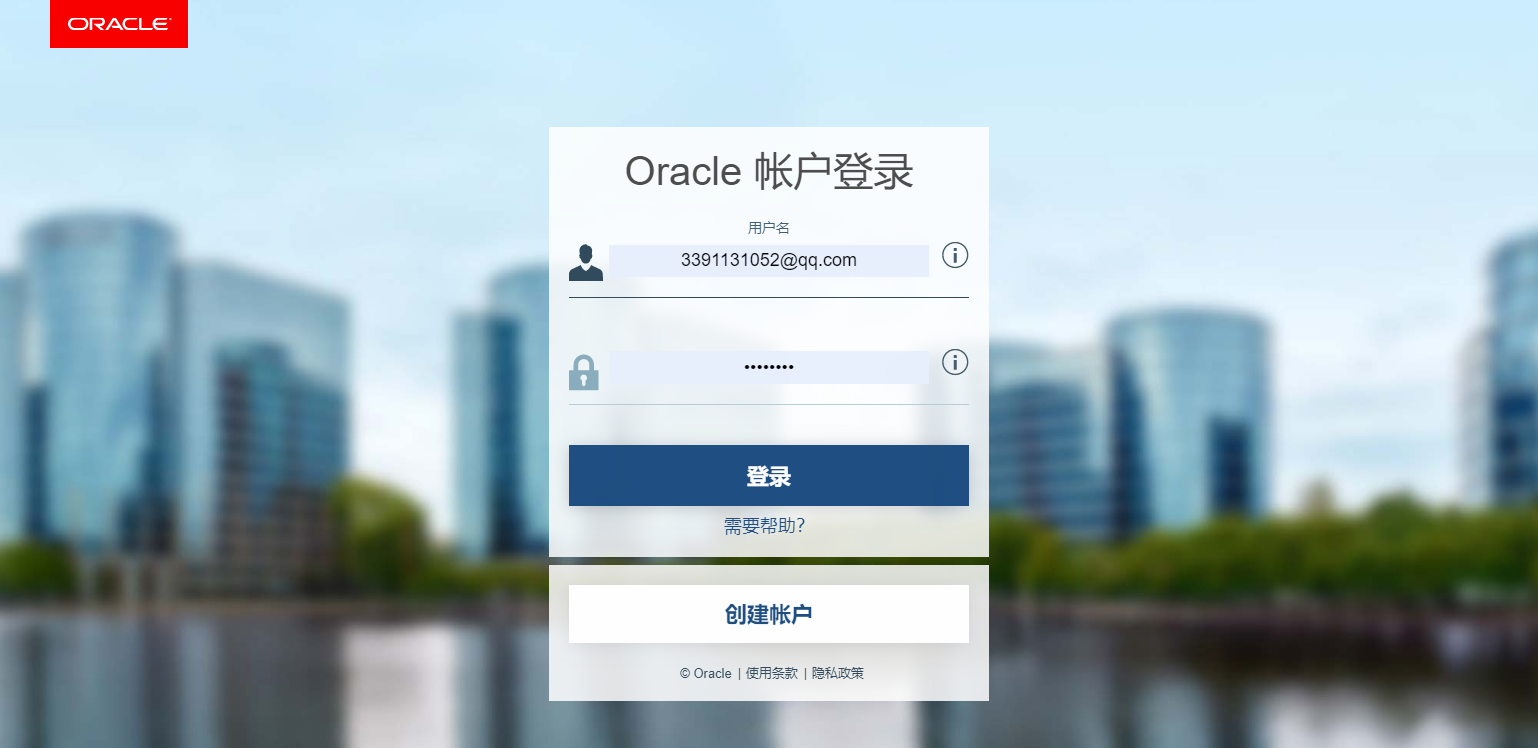
\includegraphics[width=\linewidth]{oracle.png}
	\caption{Oracle官网注册安装JDK}
	\label{fig:install_jdk}
\end{figure}


注册并下载后,完成简单的环境变量配置即可。
\lstinputlisting[style=mysh,title=安装JDK过程]{docs/scripts/install_jdk.sh}

\subsection{配置网络和SSH免密登录}
修改\lstinline{/etc/hosts}文件,添加主机名与IP地址映射关系。
\lstinputlisting[style=mysh,title=hosts文件]{docs/scripts/add_hosts.sh}
这样可以避免在其他配置的时候写硬的IP地址,
不方便修改。这样人类可读性更好。再将此文件分发到其他的几个节点上去,保持端口映射相同。
为了避免每天机器都会关闭重新启动时,\lstinline{/etc/hosts}文件被恢复,在\lstinline{/home/zhangyu}
目录下保存一份副本,每次将其覆盖即可。

在家目录下生成密钥:
\begin{lstlisting}[style=mysh]
ssh keygen	
\end{lstlisting}	
出现询问回车即可,就可以看到生成出来的公钥。

使用下列命令将秘钥复制到各个节点上。这样即可配置好免密登录。
\lstinputlisting[style=mysh,title=hosts文件]{docs/scripts/ssh-copy-id.sh}
中间出现询问和要求输入密码,输入\lstinline{yes}和密码\lstinline{zhangyu}即可。
后面测试过程中,如果正常登录且不需要输入密码,则说明配置成功了。否则需要重新配置
